\vzmstitle{О задаче гашения поперечных колебаний движущихся материалов}
\vzmsauthor{Муравей}{Л.\,А.}
\vzmsauthor{Романенков}{А.\,М.}
\vzmsinfo{Москва; {\it l\_muravey@mail.ru}; {\it romanaleks@gmail.com}}
\vzmscaption

{\bf 1.	Введение. }

Особенностью задач гашения колебаний гиперболических систем является то, что в них оптимальный режим зависит не только от времени, но и от пространственных переменных. Поэтому для нахождения минимального времени гашения колебаний и соответствующего ему оптимального уравнения используется метод сведения этой задачи к так называемой тригонометрической проблеме моментов. Наиболее значимой работой в этом направлении является статья 1983 года Д. Лагнесса [1], в которой исследовалось, в частности, возможность гашения колебаний закреплённой струны:

$$\frac{1}{a^2}w_{tt}-w_{xx}+q\left(x\right)w=g\left(x,t\right), \quad 0\leq x \leq l, \quad t > 0  \eqno{(1)}$$
Решение соответствующей смешанной задачи рассматривается как обобщённое, для которого определён интеграл энергии
$$E\left(t\right)=\int_{0}^{l}\left[w_{t}^{2}\left(x,t\right)+a^2\left(w_{x}^{2}\left(x,t\right)+q\left(x\right)w^2\left(x,t\right)\right)\right]dx, \eqno{(2)}$$
который при $g\left(x,t\right)\equiv0$, не зависит от $t$ и равен значению $E(0)$.

Задача гашения колебаний заключается в нахождении минимального значения $T_0>0$, при котором для любых допустимых начальных возмущений, найдётся управляющая функция $g_0\left(x,t\right)\in L_2(0\le x\le l,\ 0\le t\le T_0)$ (определяющая оптимальный режим), такая что:
$$E\left(T_0\right)=0, \eqno{(3)}$$
или, что тоже самое, при $g\left(x,t\right)=g_0(x,t)$ справедливо равенство:
$$\left.w\right|_{t=T_0}=0,\quad \left.w_t\right|_{t=T_0}=0 \eqno{(4)}$$

{\bf 2. Проблема моментов.}

Из закона сохранения энергии вытекает, что решение смешанной задачи при $g\left(x,t\right)=0$ представляет собой сумму так называемых «стоячих волн», которые находятся методом Фурье и имеют вид:
$$z_n(x,t)=(A_n\cos{\omega_nt+B_n\sin{\omega_nt)}}v_n\left(x\right),	\eqno{(5)}$$
здесь $v_n\left(x\right)$ -- решения соответствующей спектральной задачи, отвечающие собственным числам $\lambda_n$. При этом функции $v_n\left(x\right)$ образуют ортонормированный базис, а для собственных значений справедливо асимптотическое разложение:
$$\omega_n=a\sqrt{\lambda_n}=\frac{a\pi n}{l}+c_n+О1n,\quad n\rightarrow \infty \eqno{(6)}$$

Выполнение условий (4) для построенного методом разделения переменных решения смешанной задачи приводит нас к системе интегральных уравнений Фредгольма первого рода.
$$
{\int_{0}^{T}{u_n\left(t\right)\cos{\omega_nt\ dt=-\beta_n,\ }}
	\atop
\int_{0}^{T}{u_n\left(t\right)\sin{\omega_ntd\ t=\alpha_n\omega_n,}}
}\quad n=1,2,\ldots,	\eqno{(7)} $$
которую принято называть тригонометрической проблемой моментов. Здесь $\alpha_n,\beta_n,u_n\left(t\right)$ -- коэффициенты Фурье разложения начальных функций $\left.w\right|_{t=0}=h_0\left(x\right)$, $\left.w_t\right|_{t=0}=h_1\left(x\right)$ и правой части уравнения (1) $g(x,t)$ по ортонормированному базису $\left\{v_n\left(x\right)\right\}$. Заметим, что из (6) вытекает существование предела $\displaystyle\lim_{n\rightarrow\infty}{\frac{n}{\omega_n}=\frac{l}{\alpha\pi}}$, поэтому из результатов Н. Левинсона [2] следует, что при
$$T_0=\frac{2l}{\alpha} 	\eqno{(8)}$$
система $({\cos{\omega_nt, \sin{\omega_nt}}})$ образует базис Рисса в $L_2\left(0,T_0\right)$. Следовательно, для неё существует биортогональная система в $L_2\left(0,T_0\right)$, что позволяет установить существование единственного решения ${{u}_n^{\left(0\right)}\left(t\right)},$ (7)
а также найти оптимальное управление $g_0\left(x,t\right)$ в виде ряда Фурье

Отметим, что результаты Д. Лагнеса имеет важное значение, поскольку из них вытекает гарантированное время гашения колебаний; при этом Лагнесом было так же показано, что управляющую функцию можно использовать и в любой подобласти $\left[\gamma,\delta\right]$ отрезка $[0,l]$.

Дальнейшие работы различных авторов были посвящены приближенному решению задачи гашения колебаний и основаны на существенном сужении класса управляющих функций. При этом рассматривались струны и мембраны. Подробный обзор работ приводится в нашей монографии [3]. Кроме того, в [3] исследованы задачи гашения колебаний балок и пластин, описываемых гиперболическими по Петровскому уравнениями (в уравнение 1 входят производные четвёртого порядка по пространственным переменным). Показано, что в случае балки соответствующие собственные функции спектральной задачи почти ортогональны по Р. Беллману [4], откуда можно вывести асимптотическую разрешимость проблемы моментов. В случае же пластины показано, что двумерную тригонометрическую проблему моментов можно свести к одномерной в некотором подпространстве из $L_2\left(0,T\right)$. Отметим, что краткое изложение соответствующих результатов содержится в работе [5].

{\bf 3. Движущаяся струна.}

Целью нашей работы является решение задачи гашения поперечных колебаний продольно движущейся струны, возникающей в производстве бумажного полотна (в предположении, что полотно достаточно узкое). В монографии [6] была предложена следующая модель поперечных колебаний $w(x,t)$, связанных с движением бумажного полотна (см. рис. 1).

\begin{figure}[h]
	\center{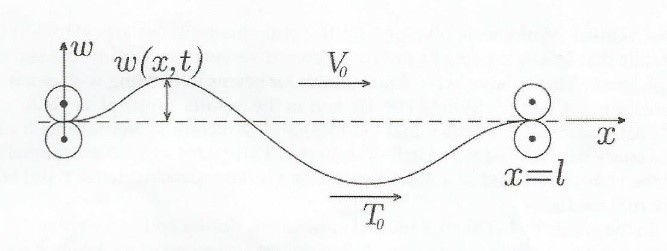
\includegraphics{1.jpg} \\Рис. 1. Профиль движущегося бумажного полотна.}
\end{figure}

$$\frac{\partial^2w}{\partial t^2}+2v_0\frac{\partial^2w}{\partial x\partial t}+\left(v_0^2-c^2\right)\frac{\partial^2w}{\partial x^2}=0,\quad 0<x<l,\quad t>0.	\eqno{(9)}$$
При этом заданы граничные условия
$$w\left(0,t\right)=w\left(l,t\right)=0,\quad t>0	\eqno{(10)}$$
и начальные возмущения:
$$w\left(x,0\right)=h_0\left(x\right),\quad w_t\left(x,0\right)=h_1\left(x\right),\quad x\in\left[0;l\right]	\eqno{(11)}$$

Для решения смешанной задачи справедлив аналогичный случаю закреплённой струны «закон сохранения энергии»:
$$\begin{array}{c}
\displaystyle E\left(t\right)= \int_{0}^{l}\left[w_t^2\left(x,t\right)+\left(c^2-v_0^2\right)w_x^2\left(x,t\right)\right]dx \equiv E(0)=\\
\displaystyle = \int_{0}^{l}{\left[h_1^2\left(x\right)+ \left(c^2-v_0^2\right){\left(h_0^\prime\left(x\right)\right)}^2\right]dx},
\end{array}\eqno{(12)}
 $$

Таким образом, кориолисово ускорение $2v_0w_{xt}$ не даёт вклада в энергию системы и в ней должно существовать решение в виде стоячих волн. Но из-за наличия члена $2v_0w_{xt}$ в (9) стоячие волны невозможно найти традиционным методом разделения переменных.


Мы будем использовать систему автомодельных решений\ $\displaystyle v_k\left(x,t\right)=\exp{\left\{\pm\frac{ik\pi}{cl}\left[v_0^2-c^2\right]t-v_0x\right\}\sin \frac{k\pi x}{l}}$, $k=1,2,\ldots$ задачи (9), (10).  Из работ [7], [8], [9] при естественном предположении $v_0<c$ вытекает, что система $\left\{v_k\left(x,0\right)\right\}$ образует базис Рисса  $\left(y_k\left(x\right),z_k\left(x\right)\right)$ в $L_2(-l,l)$.

Если управление $g\left(x,t\right)$ сосредоточено на произвольном отрезке $\left[\gamma,\delta\right]\subset[0,l]$, то в нашем случае вместо проблемы моментов (7) имеем проблему моментов

$$\left\{
 \begin{array}{c}
 \displaystyle\int_{0}^{T_0}\int_{\gamma}^{\delta}{g_0\left(x,t\right)\cos\omega_ntdxdt}={-\beta}_n,\\
 \displaystyle\int_{0}^{T_0}\int_{\gamma}^{\delta}{g_0\left(x,t\right)\sin\omega_ntdxdt}=a_n\omega_n,
 \end{array}n=1,2,\ldots,\right.
\eqno{(13)}$$
где $\omega_n=\frac{\pi n\left(c^2-v_0^2\right)}{lc},\ n=1,2,\ldots$

$$\lim_{n\rightarrow\infty}{\frac{n}{\omega_n}=\frac{lc}{\pi\left(c^2-v_0^2\right)}} \eqno{(15)}$$
а
$$T_0=\frac{2lc}{c^2-v_0^2}  \eqno{(16)}$$

Из результатов Левинсона вытекает, что тригонометрическая система в (13) образует базис Рисса в $L_2\left(0,T_0\right)$. Следовательно, для неё в $L_2\left(0,T_0\right)$ существует биортогональная система, причём искомое решение $g_0(x,t)$ системы (13) имеет вид

$$g_0\left(x,t\right)=\sum_{n=1}^{\infty}\left(A_n^2\omega_na_ny_n\left(x\right)\psi_n\left(t\right)-B_n^2\beta_nz_n\left(x\right)\right)\chi_{\left[a,\beta\right]}\left(x\right),	\eqno{(17)}$$
где $\chi_{\left[\gamma, \delta\right]}\left(x\right)$ -- характеристическая функция отрезка $\left[\gamma, \delta\right]$,

$$A_n^2=\left(\int_{\gamma}^{\delta}{y_n^2\left(x\right)dx}\right)^{-1}\quad B_n^2=\left(\int_{\gamma}^{\delta}{z_n^2\left(x\right)dx}\right)^{-1},\quad n=1,2,\ldots	\eqno{(18)}$$

Отметим, что найденное $T_0$ должно удовлетворять неравенству $T_0v_0\le l$, которое выполняется при дополнительном ограничении на $v_0$ (иначе управление <<выйдет>>  из отрезка $[0,l]$).

$$v_0\le\left(\sqrt2-1\right)c \eqno{(19)}$$

Отметим также, что некоторые результаты были получены ранее в нашей работе [10].


{\bf 4.	Построение оптимального управления.}

Будем считать, что управляющая функция $g(x,t)$ имеет вид
$$g\left(x,t\right)=\sum_{k=1}^{K}u_k(t)\chi_k(x), \eqno{(20)}$$
где $0<x_1<\dots<x_k<l$, а $\chi_k(x)$ -- характеристическая функция отрезка $[x_k-\varepsilon,x_k+\varepsilon]$, при достаточно малом $\varepsilon>0$, таком, что все указанные отрезки не пересекаются и принадлежат отрезку $[0,l]$.

Далее, определим минимизируемый функционал
$$
\begin{array}{c}
\displaystyle J_g(t)=E(t)+\lambda\int_{0}^{l}g^2(x,t)dx=\\
\displaystyle =\int_{0}^{l}\left[w_t^2(x,t)+\left(c^2-v^2_0\right)w_x^2\left(x,t\right)\right]dx+2\lambda\varepsilon\sum_{k=1}^{K}u_k^2\left(t\right)
\end{array}
\eqno{(21)}$$

Положим $2\lambda\varepsilon=\mu$ и будем считать функции $u_k(t)$ кусочно"=постоянными: $u_k(t)=u_{kp}$, при $t_{p-1}<t<t_p$, $p=1,2,\dots,P$. Здесь $P$ может принимать значения от $1$ до $N$, где $N$ -- число слоёв по времени, используемых при численном решении задачи.

Таким образом, функционал $J$ является функцией значений $u_{kp}$ и для применения градиентного метода требуется знание частных производных $\frac{\partial J}{\partial u_{xp}}, k=\overline{1,K}, p=\overline{1,P}.$ Численные расчёты, приведённые в работе~[10], показывают достаточную эффективность такого подхода.

В ряде реальных случаев ограничения на параметры задачи не выполняются и поэтому вместо задачи гашения мы рассматриваем задачу демпфирования для любого отрезка $[0,T], T<T_0$, для которой устанавливаем необходимое условие оптимальности в форме принципа максимума Л.С. Понтрягина, а именно:

 {\it если $u_k(t)$ оптимальное управление при ограничениях
	$0\leq u_k(t)\leq U$, то при каждом $t\in[0,T]$ величина
	$$\sum_{k=1}^{K}u_k(t)\int_{x_{k-1}}^{x_k}q\left(x,t\right)dx$$
	достигает своего максимума по всем $u_k(t)$, где $q(x,t)$ -- решение соответствующей сопряжённой системы.
}

В случае, когда управление зависит от $t$ и от $x$, оптимальное управление в решении задачи демпфирования может быть найдено с помощью градиентных методов условной оптимизации.

\smallskip \centerline {\bf Литература} \nopagebreak

1. {\it Lagness J.E.} Control of wave process with distributed controls supported on a subregion //SLAM Journ. Control and Optim. 1983.Vol. 1, №1. P. 68-85 https://doi.org/10.1137/0321004

2. {\it Levinson N.} Gap and density theorem //Amer. Math. Soc. Colog. Pull, vol. 26, 1940, ISBN: 978-0-8218-1026-2

3. {\it Муравей Л.А., Романенков А.М., Петров В.М.} «Оптимальное управление нелинейными процессами в задачах математической физики».2018, Изд. МАИ. ISBN 978-5-4316-0501-7

4. {\it Bellman R.} Almost orthogonal series // Amer. Math. Soc. Vol. 50, 1944

5.  {\it Атамуратов А.Ж., Михайлов И.Е., Муравей Л.А.} Проблема моментов в задачах управления упругими динамическими системами // Мехатроника, Автоматизация, Управление. 2016. Т. 17 №9.

6. {\it Banichuk N., Jeronen J., Neittaanmaki P., Saksa T., Tuovinen T.} Mehanics of moving materials. 2014, Springer, 207 p. ISBN 978-3-319-01745-7

7. {\it Muravey L.A.} On the suppression on membrane oscillations // Summaries of IUTAM Symposium <<Dynamical problems of rigid-elastic system>>. Moscow. 1990. P. 50-51

8. {\it Билалов Б.Т., Муравей Л.А.} О гашении колебаний больших механических систем // Труды международного симпозиума Intels-96. С.-Петербург. Ч.П. 1996 с. 246-254

9. {\it Билалов Б.Т.} О базисности системы $\{e^{i\alpha nx}\sin(nx)\}$ экспонент со сдвигом// ДАН РАН. 1995, т.345, №2. стр. 644-647

10. {\it Муравей Л.А., Романенков А.М., Петров В.М.} «О задаче поперечных колебаний предельно движущейся струны» // Вестник Мордовского Университета, 2018, т.28, №4. стр. 472-483
